\documentclass[xcolor=table]{beamer}

\usetheme[secheader,compress]{Madrid} %Primary theme

\usepackage{verbatim}
\usepackage{graphicx}

%% UTM Colors
\definecolor{UTMblue}{rgb}{0.043137, 0.137254, 0.254901}
\definecolor{UTMorange}{rgb}{1.0, 0.509803, 0}

\setbeamercolor{palette primary}{bg=UTMblue,fg=white}
\setbeamercolor{palette secondary}{bg=UTMblue,fg=white}
\setbeamercolor{palette tertiary}{bg=UTMblue,fg=white}
\setbeamercolor{palette quaternary}{bg=UTMblue,fg=white}
\setbeamercolor{structure}{fg=UTMblue} % itemize, enumerate, etc
\setbeamercolor{section in toc}{fg=UTMblue} % TOC sections
\setbeamercolor{title}{fg=UTMorange}

\setbeamercolor{subsection in head/foot}{bg=UTMorange,fg=white}

%%%%%%%%%%% BEGIN MACROS %%%%%%%%%%%%%%%%%%
% frameT: Frame with title
\newcommand{\frameT}[2]{\frame{\frametitle{#1} #2}}

% frameF: Fragile frame with title
\newcommand{\frameF}[2]{
  \begin{frame}[fragile]
    \frametitle{#1}
    #2
  \end{frame}
}

% frameTop: Frame aligned t the top
\newcommand{\frameTop}[2]{\frame[t]{\frametitle{#1} #2}}


\newcommand{\tab}{\hspace{1cm}}

\newcommand{\spaceor}{\hspace{5pt} \textbf{or} \hspace{5pt}}

%%%%%%%%%%% END MACROS %%%%%%%%%%%%%%%%%%%%



\begin{document}

\title{Bullet Blitz}

\author{Victor Gasior, Blade Johnson, Andrew Newbill, and Lucky Woods}
\institute{UT-Martin}
\date{\today}

%%%%%%%%%%% BEGIN TITLE %%%%%%%%%%%%%%%%%%
\frame{\titlepage}

 %\section{Outline}
%%%%%%%%%%%% END TITLE  %%%%%%%%%%%%%%%%%%


\section{Introduction}
\frameT{Motivation} {
  List some of your motivations here!
  \bigskip
  \begin{enumerate}
    \item FPS shooter game with inspiration from the game Quake
      \bigskip
    \item The idea of the game is to have players be rodent like animals like mice fighting each other with different kinds of weapons and jumping around for more movement.
  \end{enumerate}

  \bigskip
  
  \emph{ 
} \emph{ }.
}

\frameT{Technology} {
  Technology used:
  \bigskip
  \begin{enumerate}
    \item Unreal Engine 5: Used for development of the game.
      \bigskip
    \item Ultimate Doom Builder: Used for development of the maps.
    \bigskip
    \item Blender: Used for the making of the weapons in the game. 
  \end{enumerate}

  \bigskip
  
  \emph{ 
} \emph{ }.
}

\frameT{Project Goals} {
  We are wanting to make the base game with the basic gameplay working along with network connections for at least one other player to connect with the same server and a couple different maps and weapons. Goals are more weapons, more players, and possibly more unique creatures. AI enemies we are wanting to implement as well.
}

\section{Tools}

\frameT{Map Creation Pipeline} {
	\begin{center}
  		
\includegraphics[width=.8\linewidth]{figures/map_pipeline.png}
  	\end{center}
  	
  	The maps were initially made in Ultimate Doom Builder (UDB), a program meant to make Doom 2 (1994) maps. UDB supports exporting as a 3D model, however it is not properly set up for smooth importing into the Unreal Engine. In order to fix this, we imported the .obj file exported by UDB into Blender, where we then exported from Blender as a FBX file. Finally the FBX file can be imported to UE as a model.
}

\frameT{Test Maps}{
	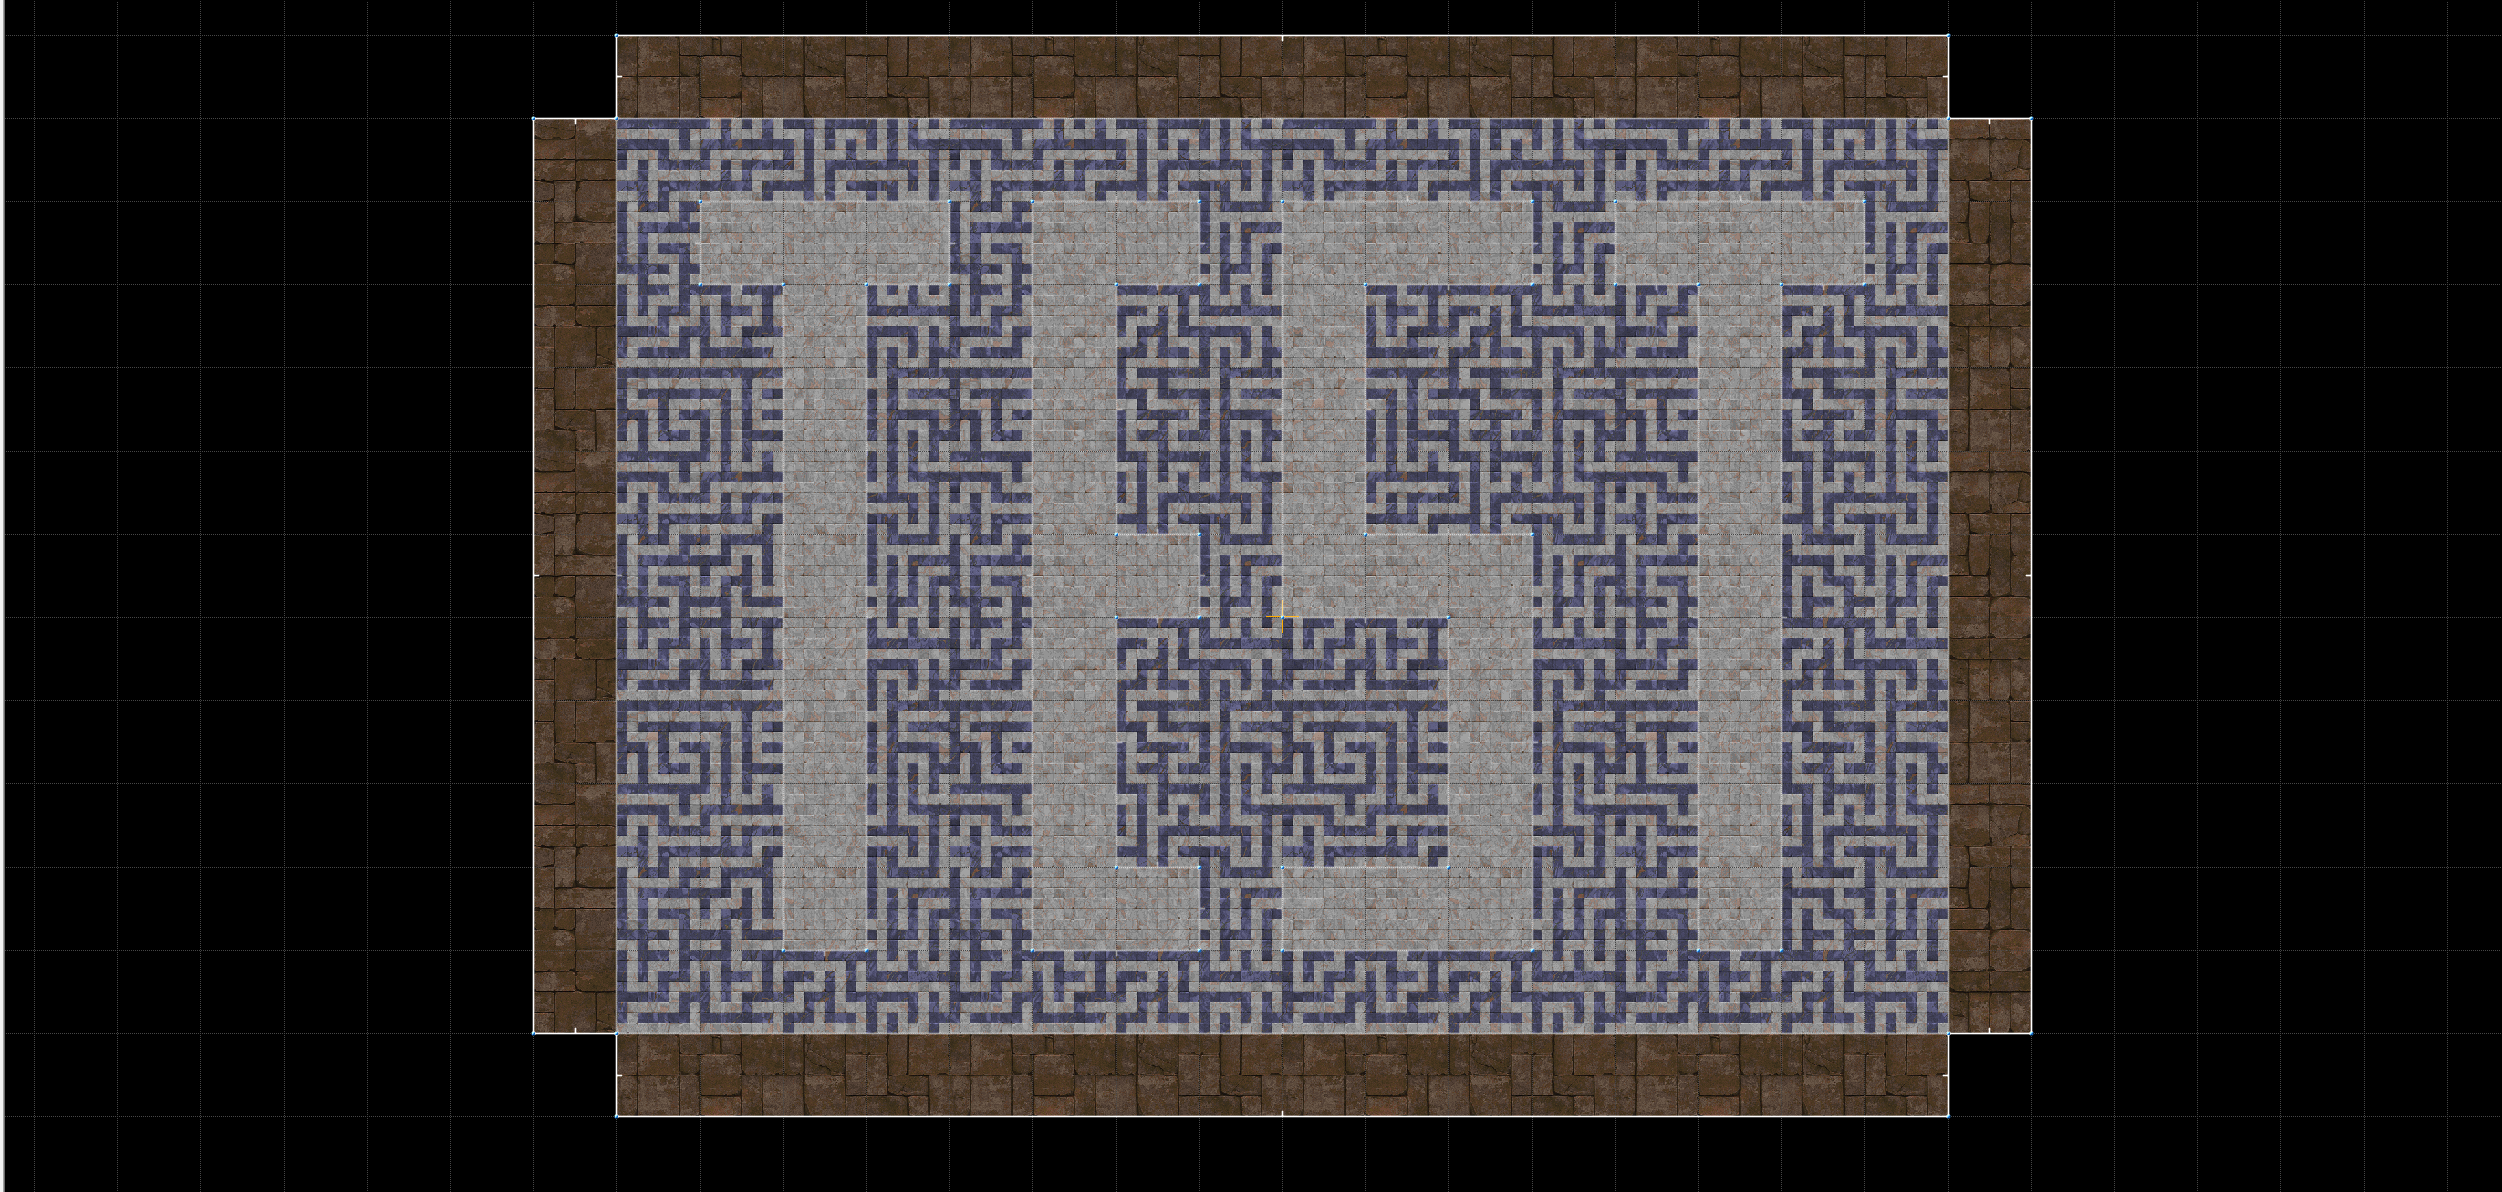
\includegraphics[height=.25\linewidth]{figures/test_map_doom.png}
	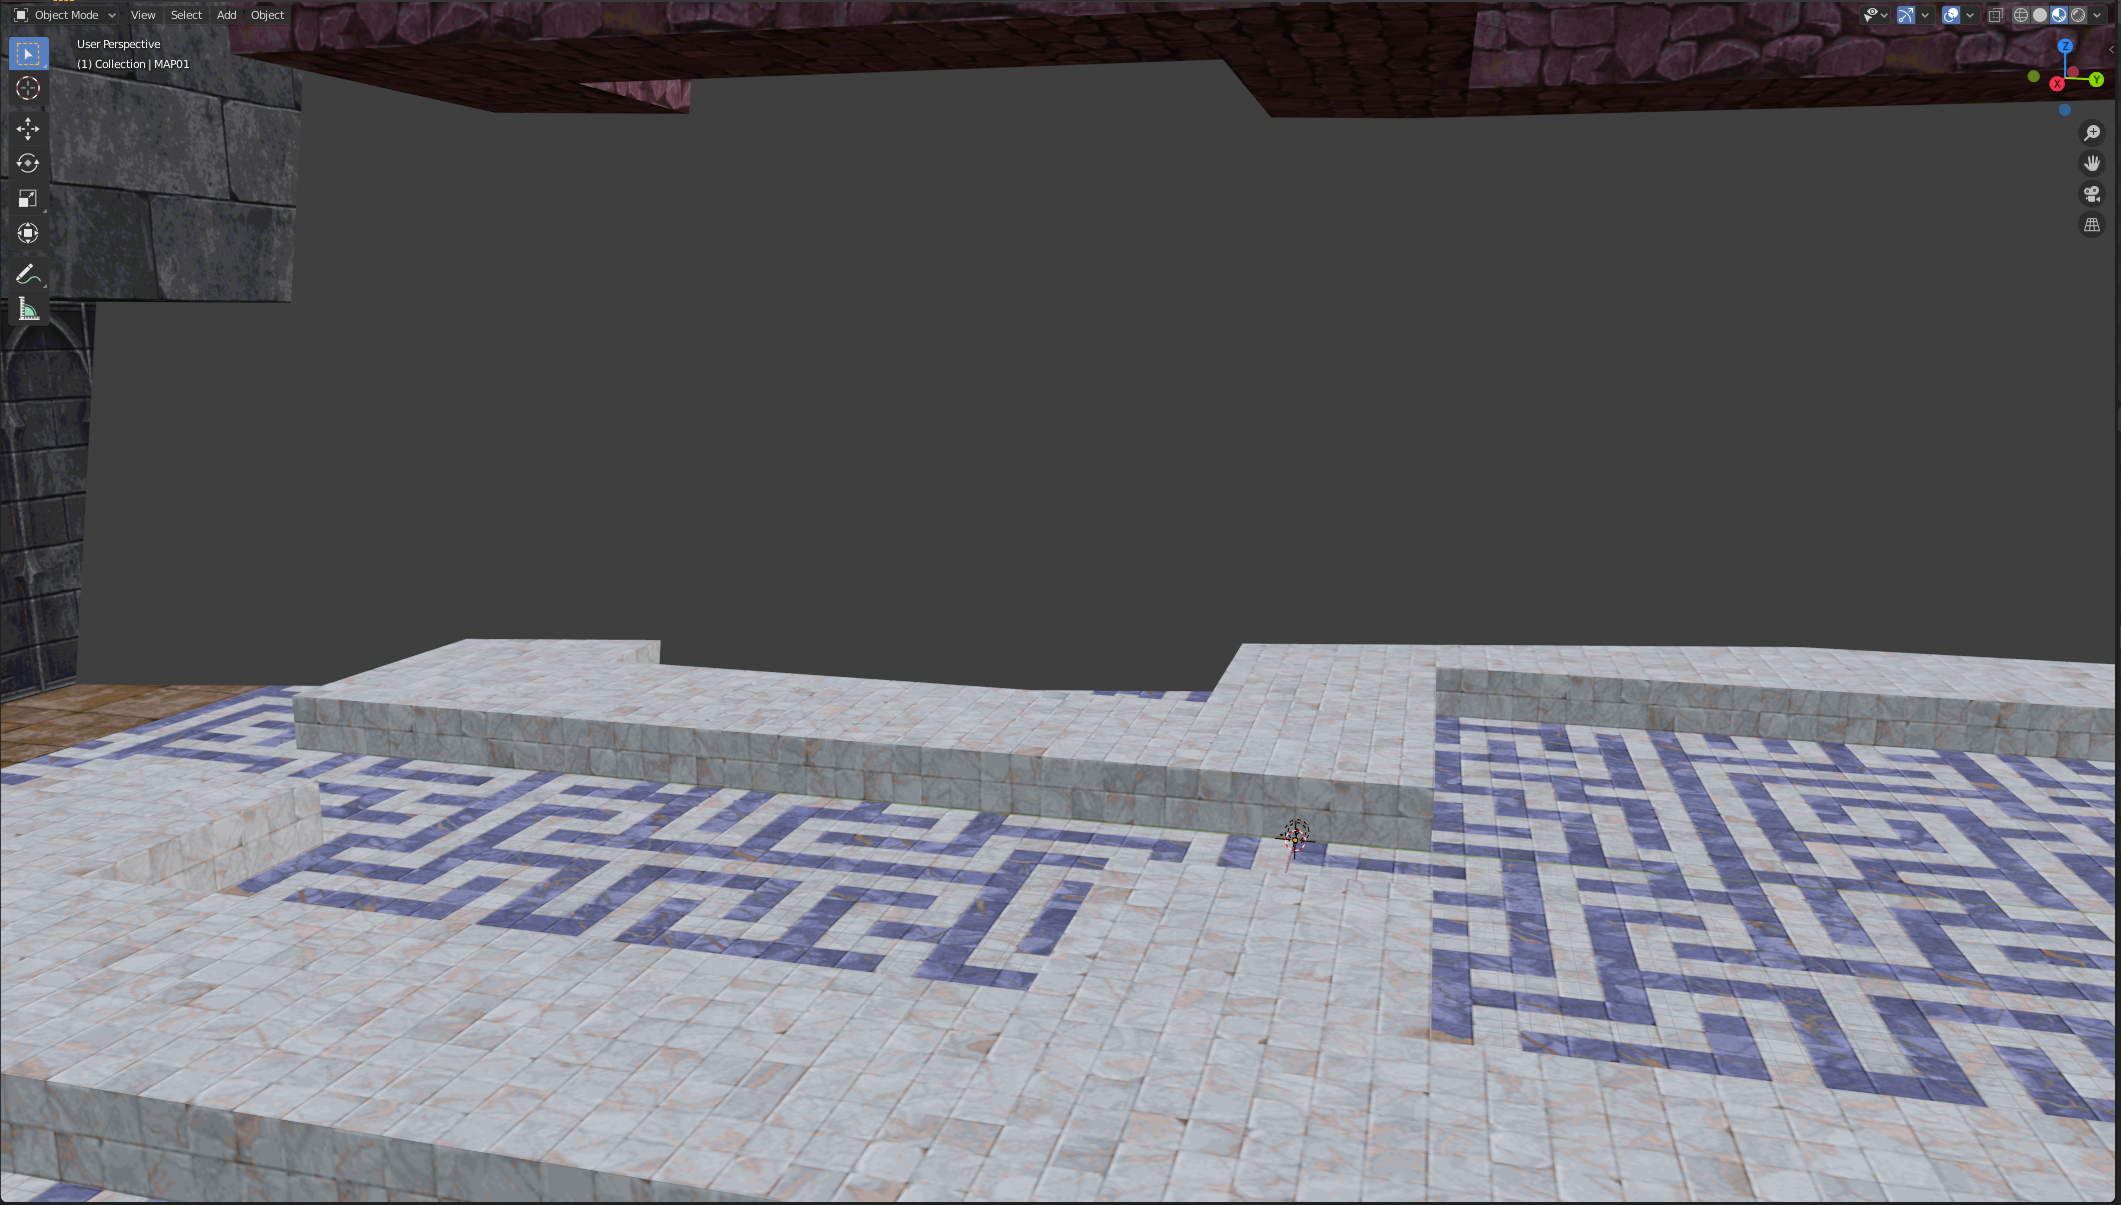
\includegraphics[height=.25\linewidth]{figures/test_map_blender.png}
	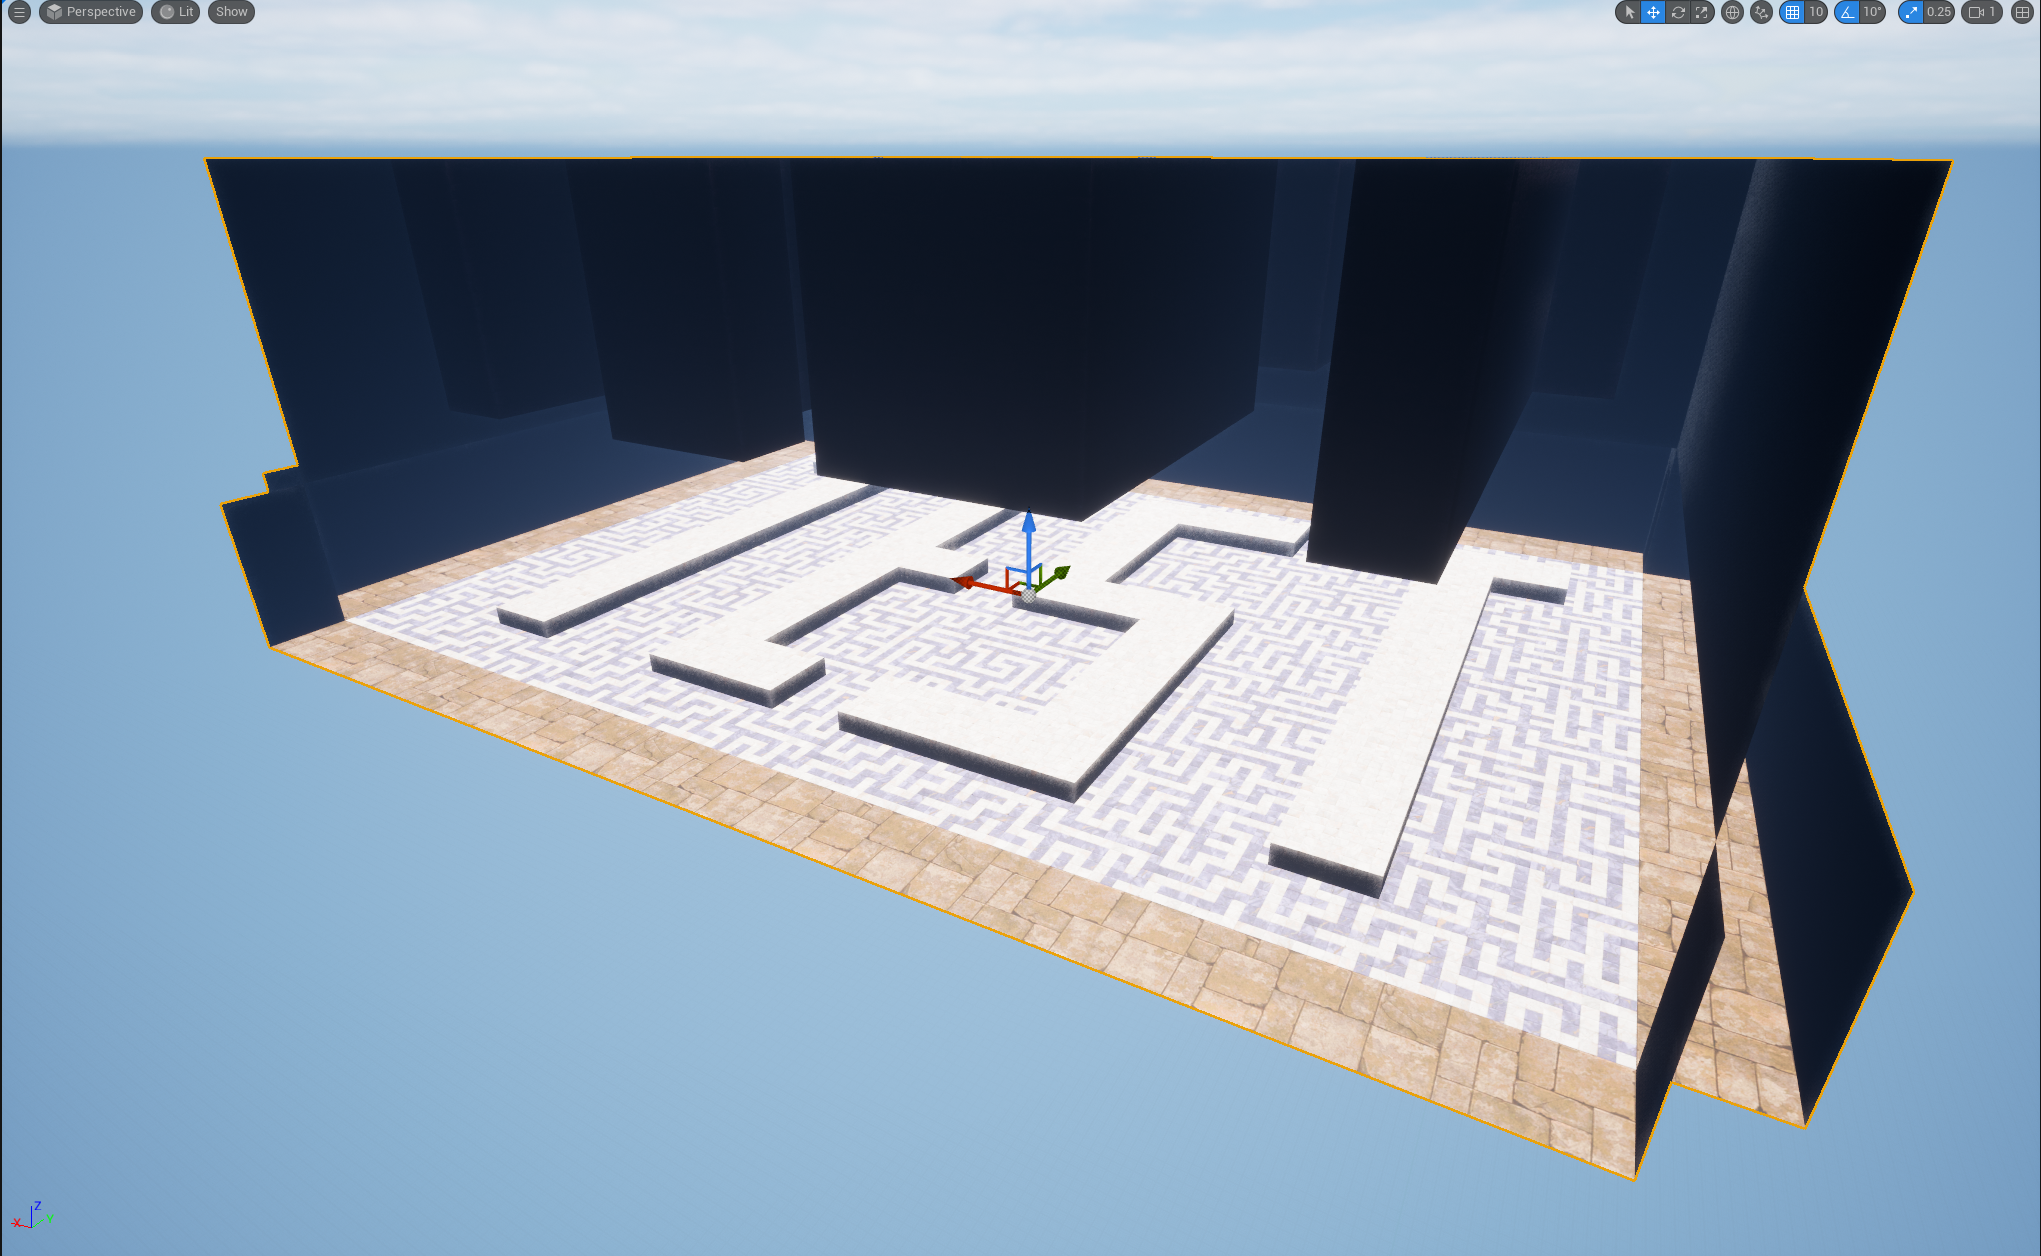
\includegraphics[height=.25\linewidth]{figures/test_map_unreal.png}
}

\frameT{Demo}{
Demo of the player in the game environment.
	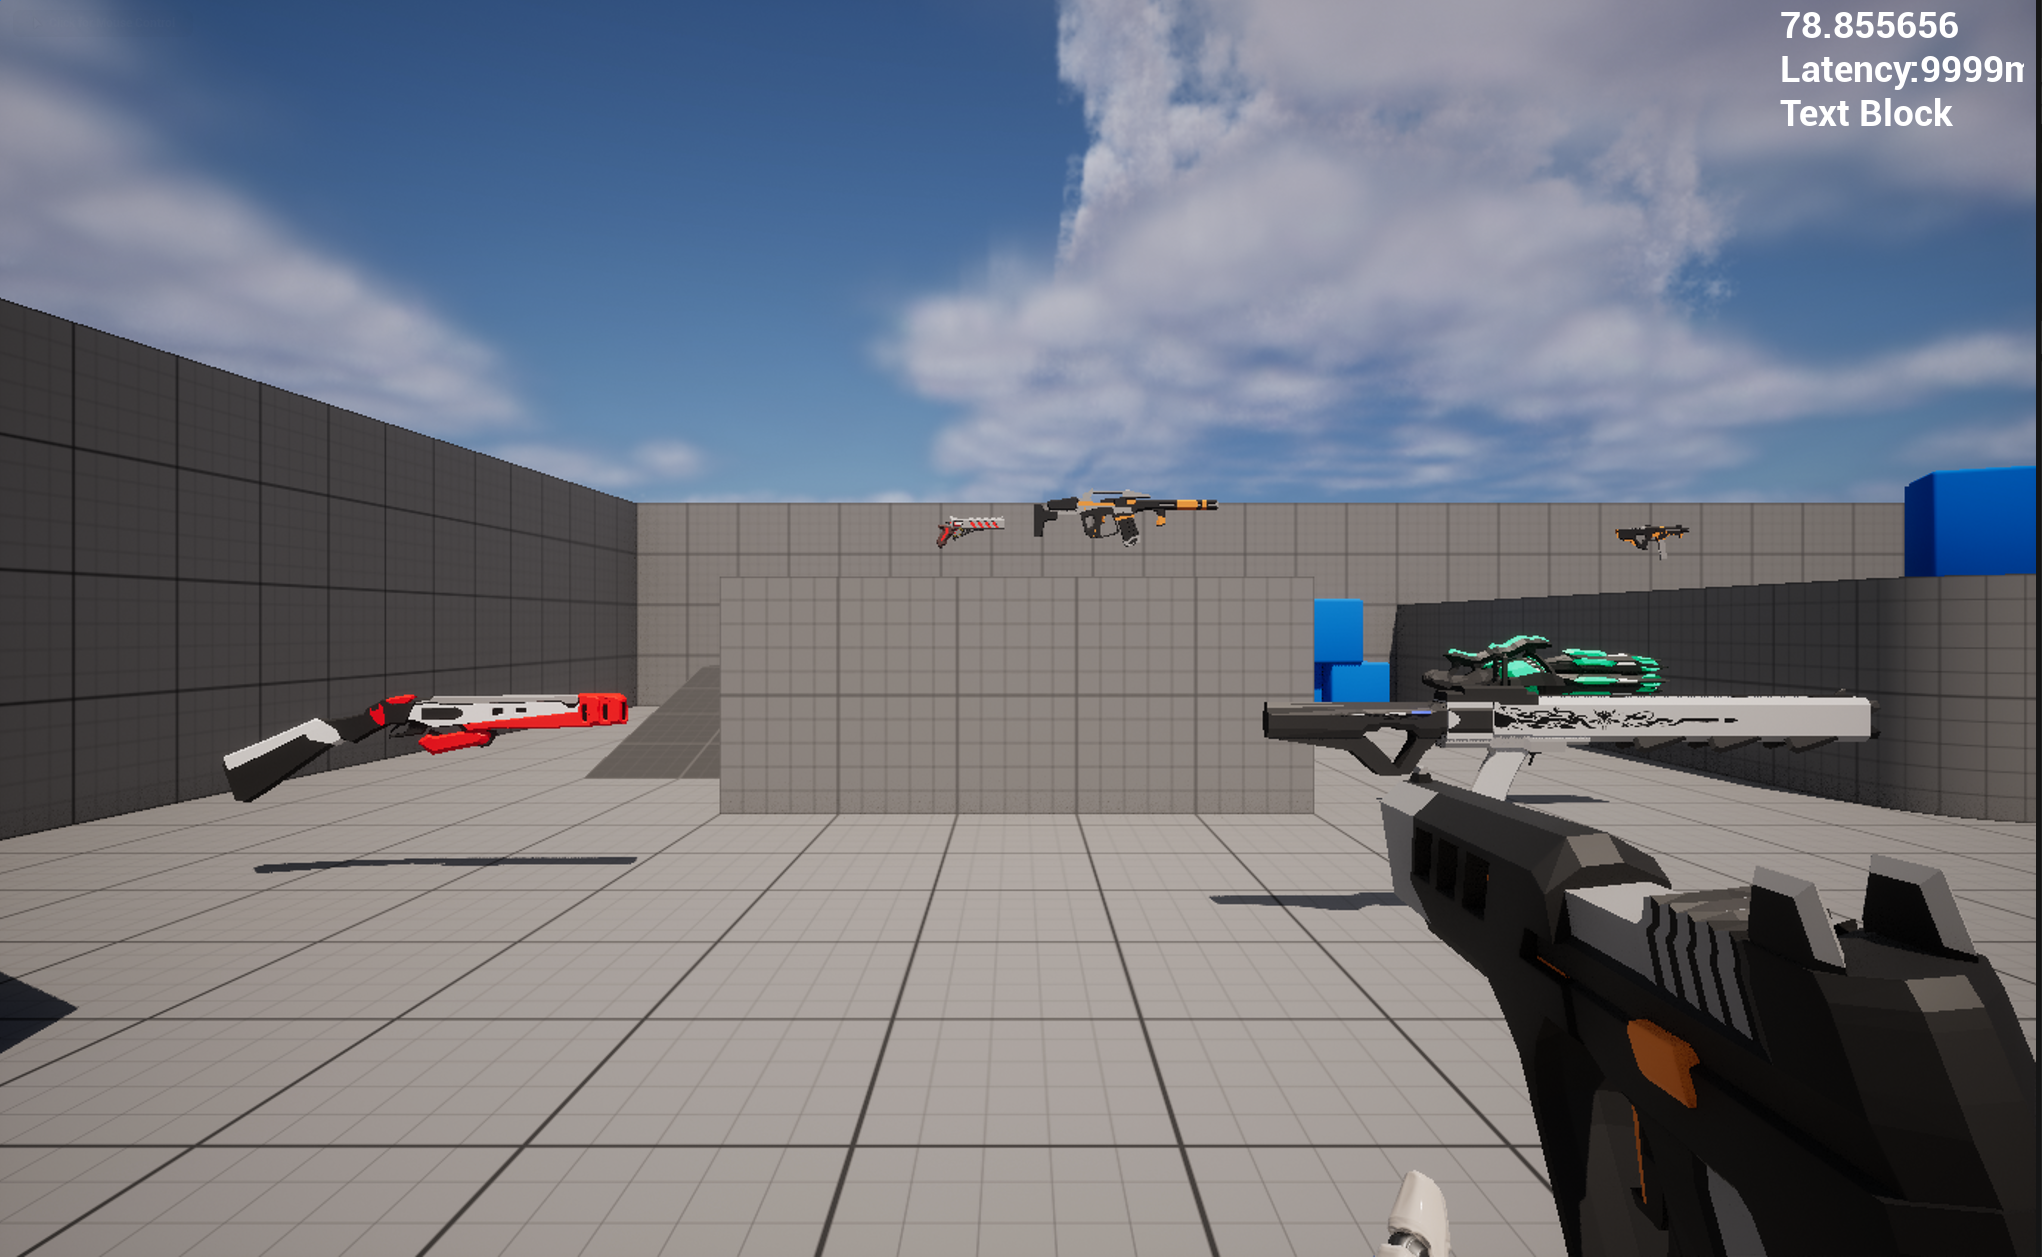
\includegraphics[height=.25\linewidth]{figures/TestDemoGame.png}
	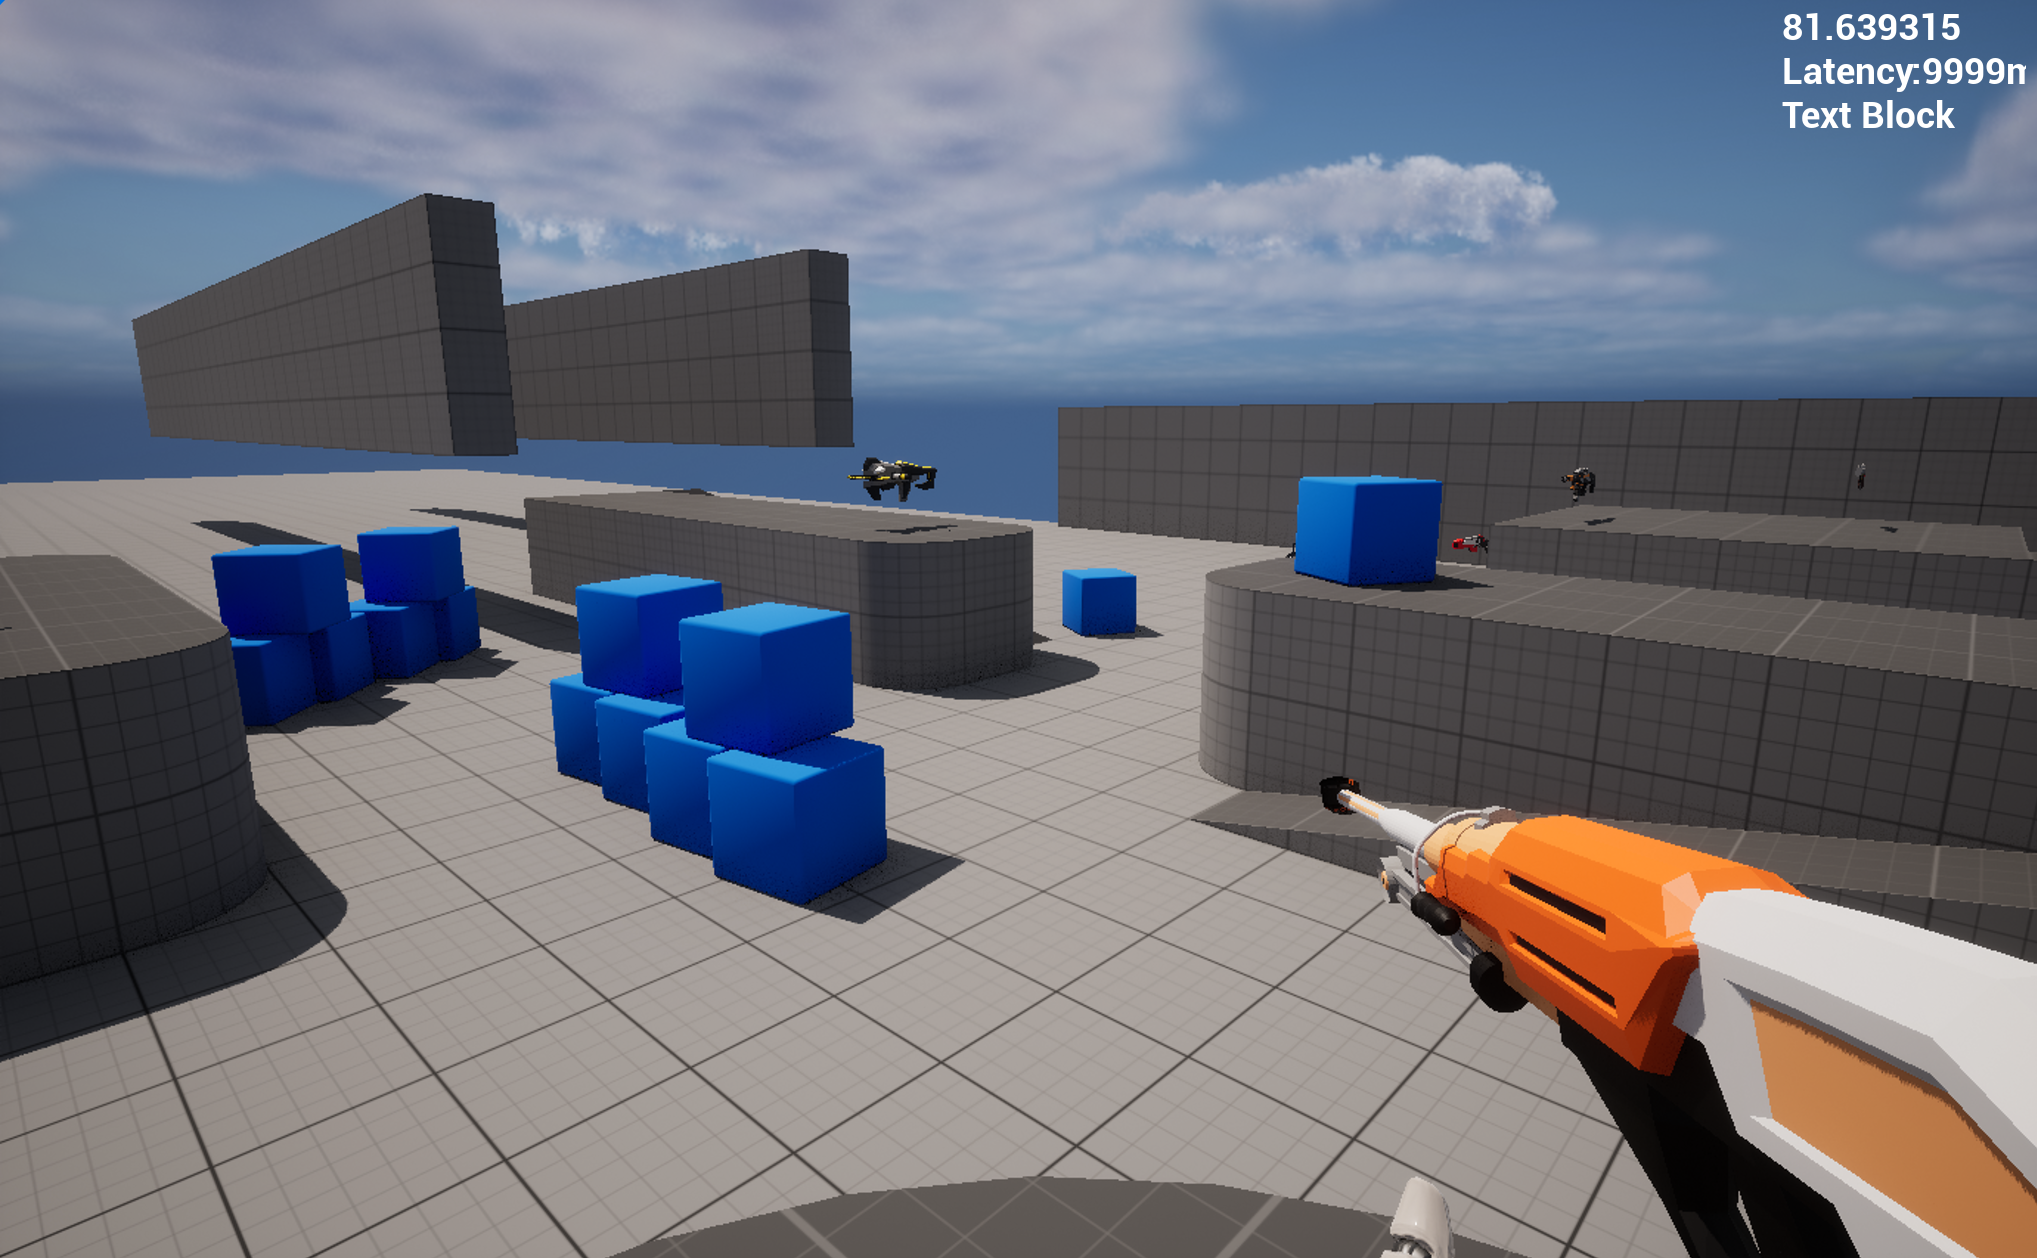
\includegraphics[height=.25\linewidth]{figures/TestDemoGame2.png}
}

\begin{frame}[fragile]
\frametitle{Family Tree Knowledge Base}
Facts:
\begin{verbatim}
Verbatim is a great way of enumerating code/algorithmic ideas.
\end{verbatim}
\end{frame}


\frameT{How to include images} {
  %% 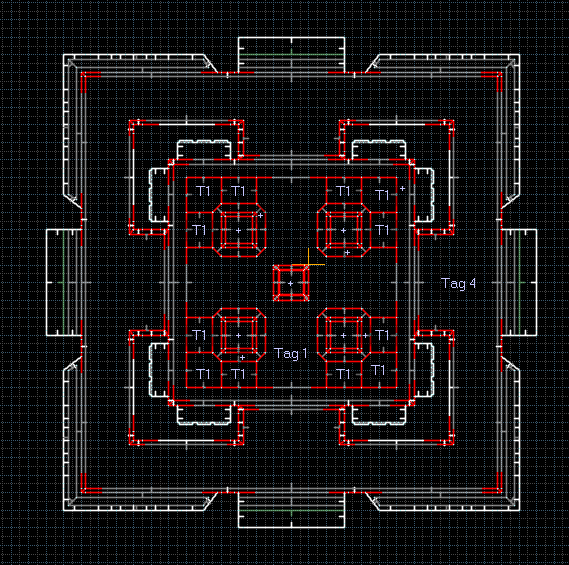
\includegraphics[width=.7\linewidth]{figures/image.pdf}
}


\begin{frame}[fragile]
  \frametitle{Social Network Graph}
  \begin{figure}[ht]
    \begin{minipage}[b]{0.53\linewidth}
      \centering
      Minipages are a great way to
    \end{minipage}
    \hspace{0.5cm}
    \begin{minipage}[b]{0.4\linewidth}
      \centering
      Line up side-by-side content.

    \end{minipage}
  \end{figure}
  
\end{frame}


\frameT{Results} {
  Describe any results of your work here.

  \bigskip

  Things that worked?

  \bigskip

  Things that didn't work?
}

\frameT{Conclusions} {
  Some bullet points here to wrap things up.
}

\frameT{Any Questions?} {
  
  \begin{center}
    Questions?
  \end{center}
  \begin{center}
    Comments?
  \end{center}

  \bigskip

  Contact Info:
\begin{enumerate}
    \item Victor Gasior: vicagasi@ut.utm.edu
      \bigskip
    \item Blade Johnson: davbjohn@ut.utm.edu
    \bigskip
    \item Andrew Newbill: andjnewb@ut.utm.edu
     \bigskip
    \item Lucky Woods: lucjwood@ut.utm.edu
\end{enumerate}

}

%\frameF{fragile test} {
%}

%% \frameF{Prolog Family Tree} {
%% \begin{verbatim}
%% hello
%% \end{verbatim}



%% }

%Empty Page
%\frameT{Frame 1}{
%}  


\end{document}
